\chapter[Texas Instruments TMS320C6678]{Texas Instruments\\TMS320C6678}
\label{chapter:c6678}
This chapter describes the Texas Instruments TMS320C6678 multicore DSP. First
the selection of the TMS320C6678 as the hardware platform for the experiments is
explained. Second the key hardware features of the platform and the related
development tools are examined.

\section{Selection of the Hardware Platform}
\fixme{intro}
The hardware platform used in the experiments in this thesis is the Advantech
TMDSEVM6678L TMS320C6678 Evaluation Module. The processor in the evaluation
module is the Texas Instruments TMS320C6678. The TMS320C6678 is a fixed and
floating point digital signal processor based on the Texas Instruments Keystone
I architecture. The processor has eight C66x DSP cores at 1.0 GHz clock
frequency \cite{tmsdatasheet}. \fixme{could be more verbose. super awkward}

The TMS320C6678 was chosen as the hardware platform for the experiments for two
main reasons. First the Keystone I architecture is designed with stream
processing applications in mind \cite{multicorevideo}. Second the objective of
this thesis is to understand hardware and software features supported by the
TMS320C6678. The specific features in the TMS320C6678 we are interested in are
the support for OpenEM included in the MCSDK for Keystone I devices
\cite{MCSDKbrochure} and the hardware accelerated scheduling and communication
utilized by the OpenEM runtime. \fixme{awkward, concise}

An additional benefit of choosing TMS320C6678 as the hardware platform for the
experiments is the support for the platform in PREESM \cite{pelcat2014preesm}.
\fixme{is this only an additional benefit?}

\section{TMS320C6678 Overview}

\begin{figure}[h!]
    \begin{center}
        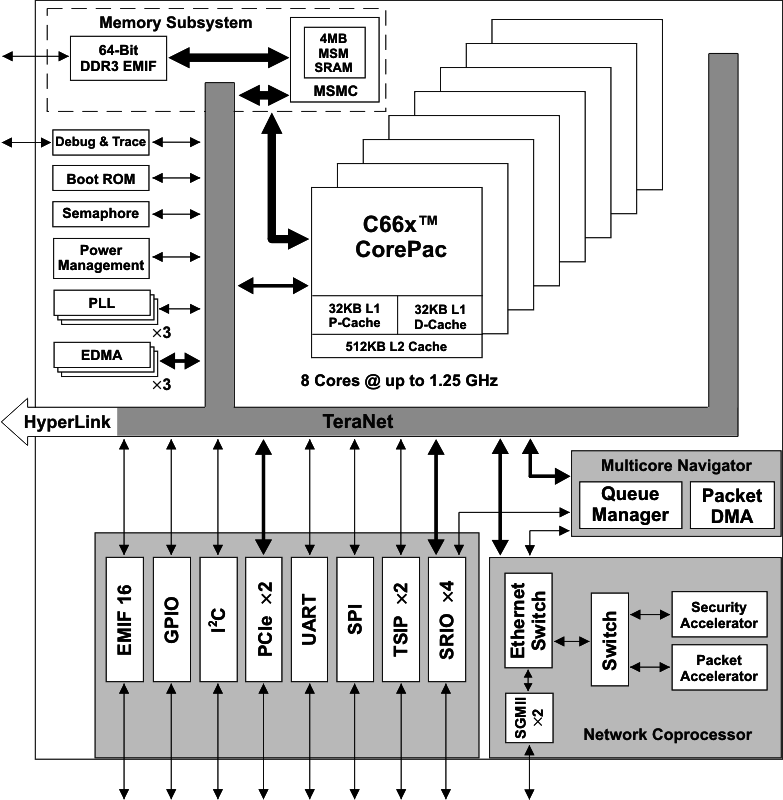
\includegraphics[width=0.99\textwidth]{images/fbd_SPRS691e.png}
        \caption{Overview of the TMS320C6678 architecture. \fixme{refer to this}}
        \label{fig:arch_overview}
    \end{center}
\end{figure}

\fixme{intro}
\fixme{what is keystone architecture? why are you talking about it?} The
Keystone I architecture the TMS320C6678 is based on specifies a set of hardware
elements which enable integration of DSP cores, application specific
co-processors and IO \cite{tmsdatasheet}. The Keystone I hardware modules and
their connections are presented in figure \ref{fig:arch_overview}. In the
Keystone I architecture there are multiple ways for the C66x cores to
communicate with each other, the memory and the peripherals. The methods of
communication of specific interest for the experiments in this thesis are
communication through shared memory discussed in \ref{subsec:c66memory} and
communication through packet based communication manager Multicore Navigator
introduced in \ref{subsec:multicorenav}.

The development board used for development of the experiment applications and
measurements was an Advantech TMDXEVM6678L. TMDXEVM6678L is an evaluation
module and hardware reference design platform for the TMS320C6678 multicore
DSP. The evaluation module provides 512 megabytes of DDR3 memory and an onboard
XDS100 emulator with USB connectivity along with other features. \cite{evmref}
The connectivity provided by the onboard emulator simplified developing and
debugging for the platform. The memory on the evaluation module helped us omit
the IO from the application design.

The IDE used for development of the experiment applications is called Code
Composer Studio. CCS version 5.2. is distributed with the evaluation module.
CCS is discussed in detail in \ref{subsec:devtools}.

\subsection{c66x DSP}
\label{subsec:c66x}
\fixme{intro}
TMS320C6678 is a multicore fixed and floating-point DSP. The device supports
core speed up to 1.4 GHz but was set up to run at 1.0 GHz for all the
experiments. The device consists of eight c66x DSPs, on-chip memory and
peripherals. The c66x is based on TMS320C66x ISA which is a VLIW architecture
with 8 functional units. The c66x CPU has 64 general-purpose 32 bit registers.
\cite{sprugh7} \fixme{a list of features. explain more}

The CPU is capable of dispatching up to eight parallel instructions every cycle.
The instructions dispatched in parallel move through pipeline stages
simultaneously. Pipelining helps eliminate CPU stalls while waiting for memory
operations or other CPU instructions taking multiple cycles complete.
\cite{sprugh7} \fixme{explain more}

\subsection{Memory}
\label{subsec:c66memory}
\fixme{intro}
The TMS320C6678 contains a multi-layer memory hierarchy which can be configured
by the user to a large extent.\fixme{how?} The memory hierarchy in the device consists of L1
and L2 memories of each core, Multicore Shared Memory (MSM) and additionally
external memory provided by the evaluation module.

Each c66x CPU has 32 KB level 1 program cache (L1P), 32 KB level 1 data cache
(L1D) and 512 KB of level 2 memory. Initially after bootup both L1P and L1D are
configured as cache but they can be reconfigured as addressable memory by
software. The L2 memory is always configured as addressable memory after reset
but can be configured as cache by software. \cite{tmsdatasheet} L2 SRAM
addresses are always cached with L1P and L1D whereas external memory addresses
are configured noncacheable by default \cite{cacheguide}.

In PC hardware cache coherence is usually handled automatically by the hardware.
In c66x, however, that is not the case. Each c66x core maintains cache coherence
between its L1 caches and the L2 cache automatically but programmer needs to
manage coherence in most other cases. For example if caching is enabled for an
external memory region shared by two cores, explicit cache coherence operations
need to be performed before each core can read from or write to the shared
region \cite{cacheguide}.

The evaluation module has 512 MB of DDR3 memory \cite{evmref}. The memory in the
evaluation module, as any external memory in other hardware configurations, is
accessible through the Multicore Shared Memory Controller (MSMC). The MSMC
itself contains 4096KB of shared memory accesible by all cores.

\subsection{Multicore Navigator}
\label{subsec:multicorenav}
\fixme{intro}
Multicore Navigator is the name for a collection of features in Keystone I and
II devices which enables hardware-accelerated, packet-based communication
between the on-chip devices. Texas Instruments claims the use of specialized
hardware for on-chip communication results in significant performance gains when
implemented carefully. Among the design goals stated for the Multicore Navigator
are minimizing host interaction and maximizing memory use efficiency.
\cite{navigator}

In Keystone I devices such as the TMS320C6678 the Multicore Navigator provides a
hardware queue manager, a special DMA access for different subsystems called
PKTDMA, for Packet DMA, and multicore host notifications via interrupts.
\cite{navigator} The Texas Instruments OpenEM implementation
\ref{chapter:openem} heavily utilizes the features provided by Multicore
Navigator. Next the Queue Manager and PKTDMA are explained.

The Queue Manager on Keystone I architecture devices is a hardware module that
manages 8192 queues. Packets are queued and removed from the queues by writing
the packet descriptors to specific memory locations. The Queue Manager is
responsible for accelerating the packet communication. In addition to the Queue
Manager the Queue Management Subsystem contains two Packed Data Structure
Processors (PSDP) which perform tasks related to the Queue Management.
\cite{navigator} For example the TI implementation of OpenEM
\ref{chapter:openem} provides its own firmware for the PDSP cores which is
utilized by the OpenEM runtime for event scheduling \cite{openemwhite}. Only one
PDSP core is used by the OpenEM runtime.

The PKTDMA is a special DMA utilized by the Multicore Navigator to transfer
packet buffers between memory locations. When a packet is sent to a queue The
PKTDMA reads the address of the data to be transferred from packet descriptor,
transfers the data in one or more data moves and writes the pointer to the data
queue specified as the receiver of the packet. \cite{navigator}

\subsection{Development Tools}
\label{subsec:devtools}
\fixme{do we need this? where to find references, ti doesn't even have a printed
CCS manual}

Texas Instruments provides a suite of tools for development on the TMS320C6678
devices. In this thesis the development tools were used through an Eclipse based
IDE called Code Composer Studio (CCS). CCS integrates source editor, compiler,
debugger, simulator and other tools. CCS version 5.2 was used in this thesis
and is available for Linux. \cite{ccspage} The thesis experiments were developed
with CCS in C89. The v8.x Texas Instruments optimizing compiler was used
\cite{compilerguide}.
